\documentclass[14pt]{extbook}
\usepackage{multicol, enumerate, enumitem, hyperref, color, soul, setspace, parskip, fancyhdr} %General Packages
\usepackage{amssymb, amsthm, amsmath, latexsym, units, mathtools} %Math Packages
\everymath{\displaystyle} %All math in Display Style
% Packages with additional options
\usepackage[headsep=0.5cm,headheight=12pt, left=1 in,right= 1 in,top= 1 in,bottom= 1 in]{geometry}
\usepackage[usenames,dvipsnames]{xcolor}
\usepackage{dashrule}  % Package to use the command below to create lines between items
\newcommand{\litem}[1]{\item#1\hspace*{-1cm}\rule{\textwidth}{0.4pt}}
\pagestyle{fancy}
\lhead{Progress Quiz 2}
\chead{}
\rhead{Version A}
\lfoot{4389-3341}
\cfoot{}
\rfoot{Summer C 2021}
\begin{document}

\begin{enumerate}
\litem{
Solve the quadratic equation below. Then, choose the intervals that the solutions belong to, with $x_1 \leq x_2$ (if they exist).\[ -11x^{2} -9 x + 4 = 0 \]\begin{enumerate}[label=\Alph*.]
\item \( x_1 \in [-1.28, -1.09] \text{ and } x_2 \in [-0.5, 0.7] \)
\item \( x_1 \in [-3.72, -3.35] \text{ and } x_2 \in [12, 14.5] \)
\item \( x_1 \in [-0.89, 0.42] \text{ and } x_2 \in [1.1, 2.7] \)
\item \( x_1 \in [-16.89, -16.06] \text{ and } x_2 \in [15.5, 16.3] \)
\item \( \text{There are no Real solutions.} \)

\end{enumerate} }
\litem{
Factor the quadratic below. Then, choose the intervals that contain the constants in the form $(ax+b)(cx+d); b \leq d.$\[ 16x^{2} +24 x + 9 \]\begin{enumerate}[label=\Alph*.]
\item \( a \in [1.76, 2.61], \hspace*{5mm} b \in [0, 4], \hspace*{5mm} c \in [7.67, 8.57], \text{ and } \hspace*{5mm} d \in [0, 7] \)
\item \( a \in [0.23, 1.18], \hspace*{5mm} b \in [9, 17], \hspace*{5mm} c \in [0.55, 1.74], \text{ and } \hspace*{5mm} d \in [10, 15] \)
\item \( a \in [6.8, 8.12], \hspace*{5mm} b \in [0, 4], \hspace*{5mm} c \in [1.38, 2.63], \text{ and } \hspace*{5mm} d \in [0, 7] \)
\item \( a \in [3.19, 5.11], \hspace*{5mm} b \in [0, 4], \hspace*{5mm} c \in [3.7, 4.25], \text{ and } \hspace*{5mm} d \in [0, 7] \)
\item \( \text{None of the above.} \)

\end{enumerate} }
\litem{
Graph the equation below.\[ f(x) = (x-3)^2 - 16 \]\begin{enumerate}[label=\Alph*.]
\begin{multicols}{2}\item 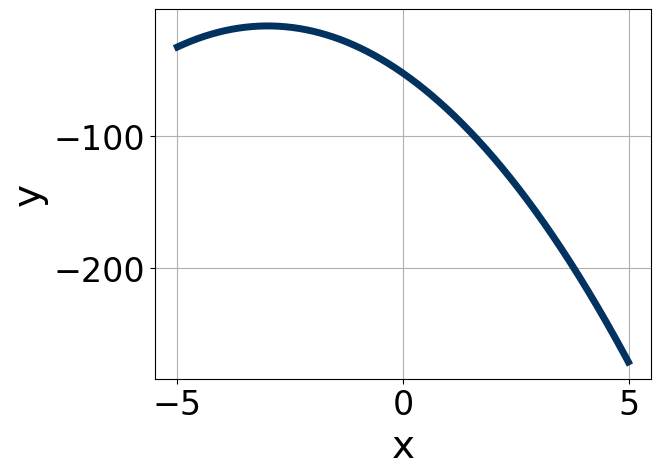
\includegraphics[width = 0.3\textwidth]{../Figures/quadraticEquationToGraphCopyAA.png}\item 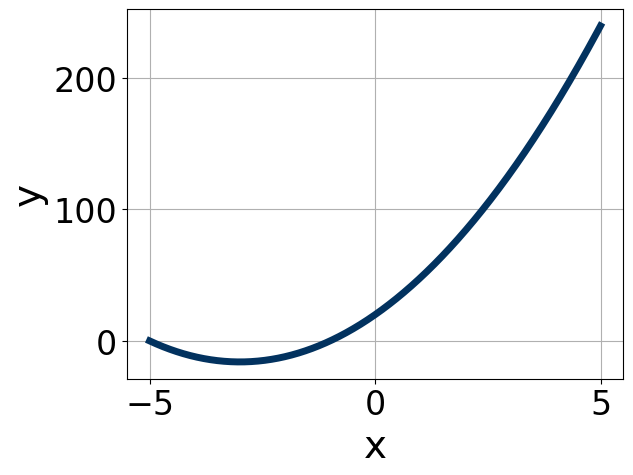
\includegraphics[width = 0.3\textwidth]{../Figures/quadraticEquationToGraphCopyBA.png}\item 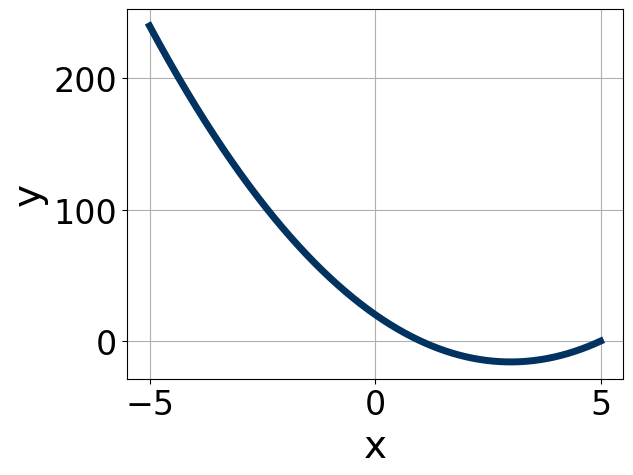
\includegraphics[width = 0.3\textwidth]{../Figures/quadraticEquationToGraphCopyCA.png}\item 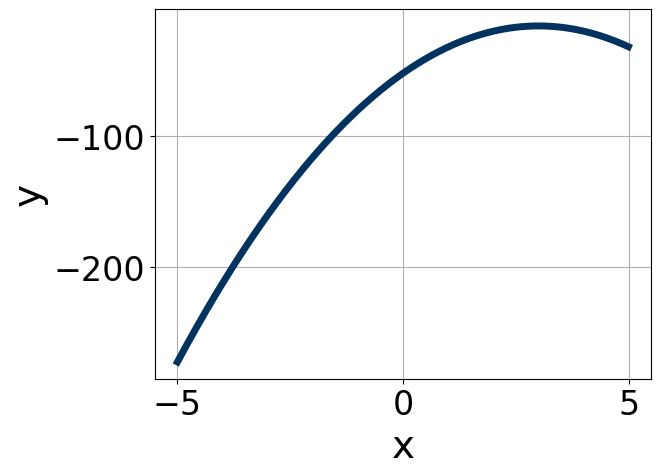
\includegraphics[width = 0.3\textwidth]{../Figures/quadraticEquationToGraphCopyDA.png}\end{multicols}\item None of the above.
\end{enumerate} }
\litem{
Graph the equation below.\[ f(x) = (x+1)^2 - 18 \]\begin{enumerate}[label=\Alph*.]
\begin{multicols}{2}\item 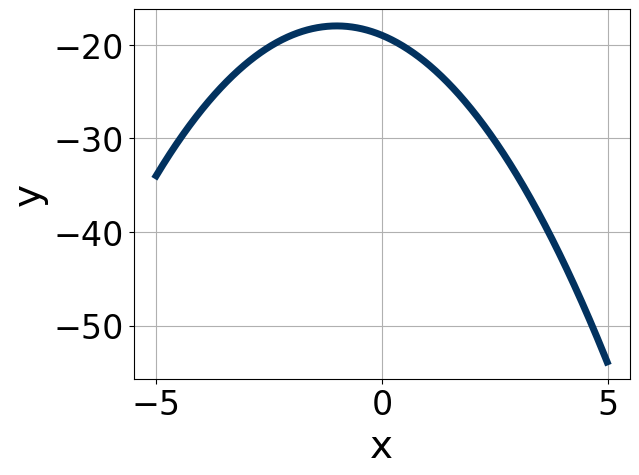
\includegraphics[width = 0.3\textwidth]{../Figures/quadraticEquationToGraphAA.png}\item 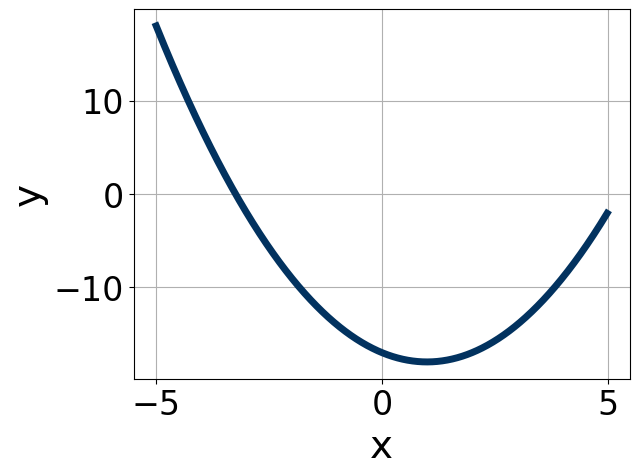
\includegraphics[width = 0.3\textwidth]{../Figures/quadraticEquationToGraphBA.png}\item 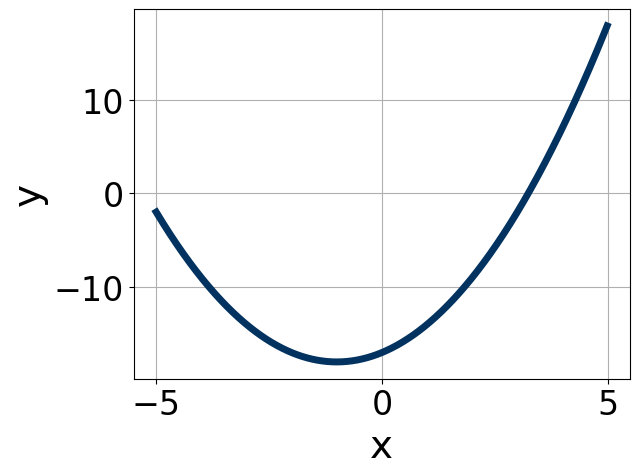
\includegraphics[width = 0.3\textwidth]{../Figures/quadraticEquationToGraphCA.png}\item 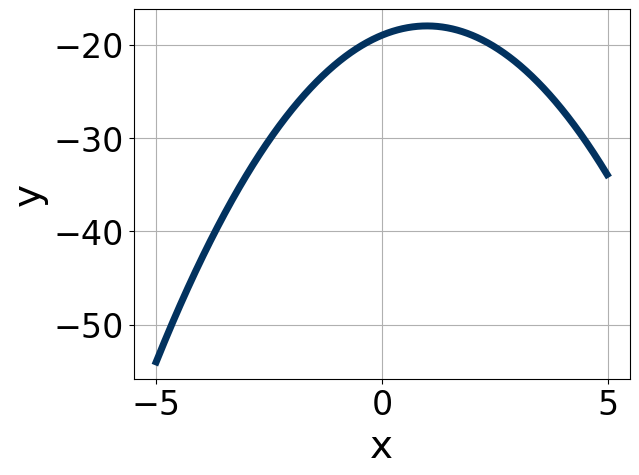
\includegraphics[width = 0.3\textwidth]{../Figures/quadraticEquationToGraphDA.png}\end{multicols}\item None of the above.
\end{enumerate} }
\litem{
Solve the quadratic equation below. Then, choose the intervals that the solutions belong to, with $x_1 \leq x_2$ (if they exist).\[ 14x^{2} -14 x -9 = 0 \]\begin{enumerate}[label=\Alph*.]
\item \( x_1 \in [-0.71, -0.11] \text{ and } x_2 \in [1.1, 4.1] \)
\item \( x_1 \in [-6.29, -5.55] \text{ and } x_2 \in [18.1, 21.6] \)
\item \( x_1 \in [-26.62, -25.55] \text{ and } x_2 \in [23.9, 28.9] \)
\item \( x_1 \in [-2.38, -1.09] \text{ and } x_2 \in [-1.1, 0.9] \)
\item \( \text{There are no Real solutions.} \)

\end{enumerate} }
\litem{
Write the equation of the graph presented below in the form $f(x)=ax^2+bx+c$, assuming  $a=1$ or $a=-1$. Then, choose the intervals that $a, b,$ and $c$ belong to.
\begin{center}
    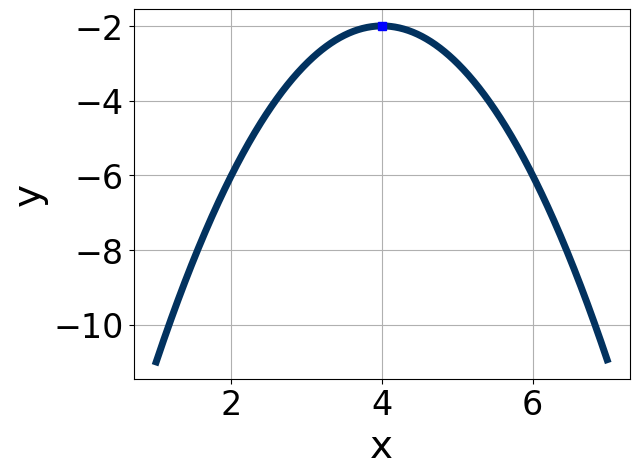
\includegraphics[width=0.5\textwidth]{../Figures/quadraticGraphToEquationA.png}
\end{center}
\begin{enumerate}[label=\Alph*.]
\item \( a \in [-0.2, 2.2], \hspace*{5mm} b \in [8, 12], \text{ and } \hspace*{5mm} c \in [14, 16] \)
\item \( a \in [-0.2, 2.2], \hspace*{5mm} b \in [-9, -7], \text{ and } \hspace*{5mm} c \in [14, 16] \)
\item \( a \in [-1.6, 0.9], \hspace*{5mm} b \in [-9, -7], \text{ and } \hspace*{5mm} c \in [-18, -17] \)
\item \( a \in [-1.6, 0.9], \hspace*{5mm} b \in [-9, -7], \text{ and } \hspace*{5mm} c \in [-16, -9] \)
\item \( a \in [-1.6, 0.9], \hspace*{5mm} b \in [8, 12], \text{ and } \hspace*{5mm} c \in [-18, -17] \)

\end{enumerate} }
\litem{
Solve the quadratic equation below. Then, choose the intervals that the solutions $x_1$ and $x_2$ belong to, with $x_1 \leq x_2$.\[ 25x^{2} +65 x + 36 = 0 \]\begin{enumerate}[label=\Alph*.]
\item \( x_1 \in [-9.06, -8.32] \text{ and } x_2 \in [-0.18, -0.1] \)
\item \( x_1 \in [-2.41, -1.75] \text{ and } x_2 \in [-0.83, -0.78] \)
\item \( x_1 \in [-45.56, -44.72] \text{ and } x_2 \in [-20.11, -19.97] \)
\item \( x_1 \in [-5.64, -5.34] \text{ and } x_2 \in [-0.28, -0.2] \)
\item \( x_1 \in [-1.79, -1.48] \text{ and } x_2 \in [-0.93, -0.87] \)

\end{enumerate} }
\litem{
Factor the quadratic below. Then, choose the intervals that contain the constants in the form $(ax+b)(cx+d); b \leq d.$\[ 36x^{2} -60 x + 25 \]\begin{enumerate}[label=\Alph*.]
\item \( a \in [4.1, 7.1], \hspace*{5mm} b \in [-13, 3], \hspace*{5mm} c \in [4.6, 6.4], \text{ and } \hspace*{5mm} d \in [-10, -3] \)
\item \( a \in [10.6, 13], \hspace*{5mm} b \in [-13, 3], \hspace*{5mm} c \in [1.7, 3.5], \text{ and } \hspace*{5mm} d \in [-10, -3] \)
\item \( a \in [-2.1, 1.1], \hspace*{5mm} b \in [-31, -25], \hspace*{5mm} c \in [0, 2.2], \text{ and } \hspace*{5mm} d \in [-30, -24] \)
\item \( a \in [2, 3.3], \hspace*{5mm} b \in [-13, 3], \hspace*{5mm} c \in [10.4, 14.2], \text{ and } \hspace*{5mm} d \in [-10, -3] \)
\item \( \text{None of the above.} \)

\end{enumerate} }
\litem{
Write the equation of the graph presented below in the form $f(x)=ax^2+bx+c$, assuming  $a=1$ or $a=-1$. Then, choose the intervals that $a, b,$ and $c$ belong to.
\begin{center}
    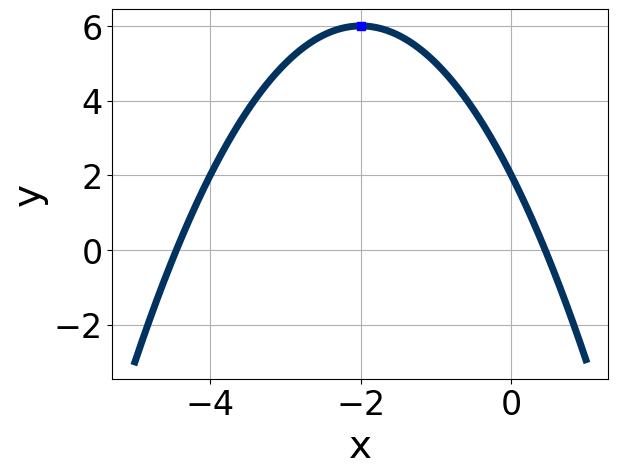
\includegraphics[width=0.5\textwidth]{../Figures/quadraticGraphToEquationCopyA.png}
\end{center}
\begin{enumerate}[label=\Alph*.]
\item \( a \in [0, 4], \hspace*{5mm} b \in [-6, -2], \text{ and } \hspace*{5mm} c \in [8, 11] \)
\item \( a \in [-3, 0], \hspace*{5mm} b \in [4, 6], \text{ and } \hspace*{5mm} c \in [-11, -7] \)
\item \( a \in [-3, 0], \hspace*{5mm} b \in [4, 6], \text{ and } \hspace*{5mm} c \in [0, 5] \)
\item \( a \in [0, 4], \hspace*{5mm} b \in [4, 6], \text{ and } \hspace*{5mm} c \in [8, 11] \)
\item \( a \in [-3, 0], \hspace*{5mm} b \in [-6, -2], \text{ and } \hspace*{5mm} c \in [0, 5] \)

\end{enumerate} }
\litem{
Solve the quadratic equation below. Then, choose the intervals that the solutions $x_1$ and $x_2$ belong to, with $x_1 \leq x_2$.\[ 15x^{2} +7 x -36 = 0 \]\begin{enumerate}[label=\Alph*.]
\item \( x_1 \in [-1.4, 0.26] \text{ and } x_2 \in [3.9, 4.44] \)
\item \( x_1 \in [-27.42, -25.33] \text{ and } x_2 \in [19.3, 20.36] \)
\item \( x_1 \in [-2.55, -0.86] \text{ and } x_2 \in [1.33, 1.38] \)
\item \( x_1 \in [-9.22, -8.23] \text{ and } x_2 \in [-0.64, 0.39] \)
\item \( x_1 \in [-4.63, -2.83] \text{ and } x_2 \in [0.31, 1.16] \)

\end{enumerate} }
\end{enumerate}

\end{document}